\begin{problem}{Longest Increasing Subsequnce}
    Given an integer array nums, return the length of the longest strictly increasing subsequence. LC 300\\
    (a)Give $O(n^2)$ algorithm.\\
    (b)Give $O(n*log(n))$ algorithm.
\end{problem}

\begin{solution}[Inclusion-Exclusion]
    \vspace{2mm}
    \hrule
    \vspace{2mm}

    Standard recursive solution.
    let $f(idx,\_)$:= maximum lis length when we are allowed to chose element from [0...idx] \textbf{only}.

    \medskip
    Considerting we have answer for our subproblem.\\
    Then at index idx, we can fill up sarr[idx] in following ways:\\
    (a) pick arr[idx] if it satify the constrain\\
    (b) do not pick arr[idx]\\

    \begin{verbatim}
        int findAns(int idx,int last,vector<int> &sarr,const vector<int>&arr)
        {
            if(idx >= arr.size())
                return 0;
            
            /* for analysing the solution being created*\
    cc        printf("\t::[%d]: last(%d)\t",idx,last);
    cc        for(auto k:sarr) cout<<k<<" ";
    cc        cout<<endl;
                  
            int inc = 0; //Explain: why inc=1 is not the defult value?
            int exc = 0;
            
            if(last < arr[idx])
            {
                sarr.push_back(arr[idx]);
                inc = 1 + findAns(idx+1,arr[idx],sarr,arr);
                sarr.pop_back();
            }
            
            exc = findAns(idx+1,last,sarr,arr);   
            /* for analysing the optimal option to chose at index idx*/    
    cc      printf("[%d]:(%d,%d)\n",idx,inc,exc);
            
            return max(inc,exc);           
        }
    \end{verbatim}

    Follow-Up Question:\\
        (a) In case last in very big, how will you modify your solution so that its memoization is within time limit? (sol: see findAnsTwo)\\
        (b) Modify the solution of (a) and shift the invalid detection condition to recursion base condition. (sol: findAnsThree)

\end{solution}

\begin{solution}[Ending at idx]
    \obeylines
    \obeyspaces
    This is one of the DP approach where we will build the solution in iterative fashion.

    let dp[idx] := lenght of maximum lis \textbf{ending at idx.}
    \medskip
    Considering case when dp[0...idx-1] is know:
    Then for dp[idx], we can pair this up with all the dp[0...idx-1]. (with constrain satisfied)

    \begin{verbatim}
        int LISViaDP(vector<int>& arr)
        {
            int size = arr.size();
            
            vector<int> dp(size,1); //dp[idx] := lenght of longest lis which is ending at idx.
            
            for(int i=1;i<size;i++)
            {
                for(int j=0;j<i;j++)
                {
                    if(arr[i] > arr[j])
                        dp[i] = max(dp[i] , dp[j] + 1);
                }
            }
            
            int mx = 0;
            for(int i=0;i<dp.size();i++)
                mx = max(mx,dp[i]); 
            
            return mx;
        }
    \end{verbatim}
    

\end{solution}

\begin{solution}[Patience Sorting | $O(n*log(n))$]
    DP + Greedy\\
    Following up with the above solution.
    
    $dp[idx] = max(dp[idx] , 1+dp[j]) \forall \text{ j such that } arr[j] < arr[idx]$\\
    Can you the guess the subproblem dp[j] (for j<idx) which will give us the best result??

    \medskip
    Q: Out of various subproblem,can you chose specifc one \textbf{greedly}?? \newline

    \smallskip
    S: This is done by PatienceSorting algorithm first proposed by Hammersley.\\ In PatienceSorting, we maintain a seperate list of stack of cards.
        At each step we take an element from arr[] from left to right. Then try to place it on stack of cards availalbe.
        The stack is decreasing sequence.\\
        % TO-DO: add diagram: 
        
        \begin{figure}[ht]
        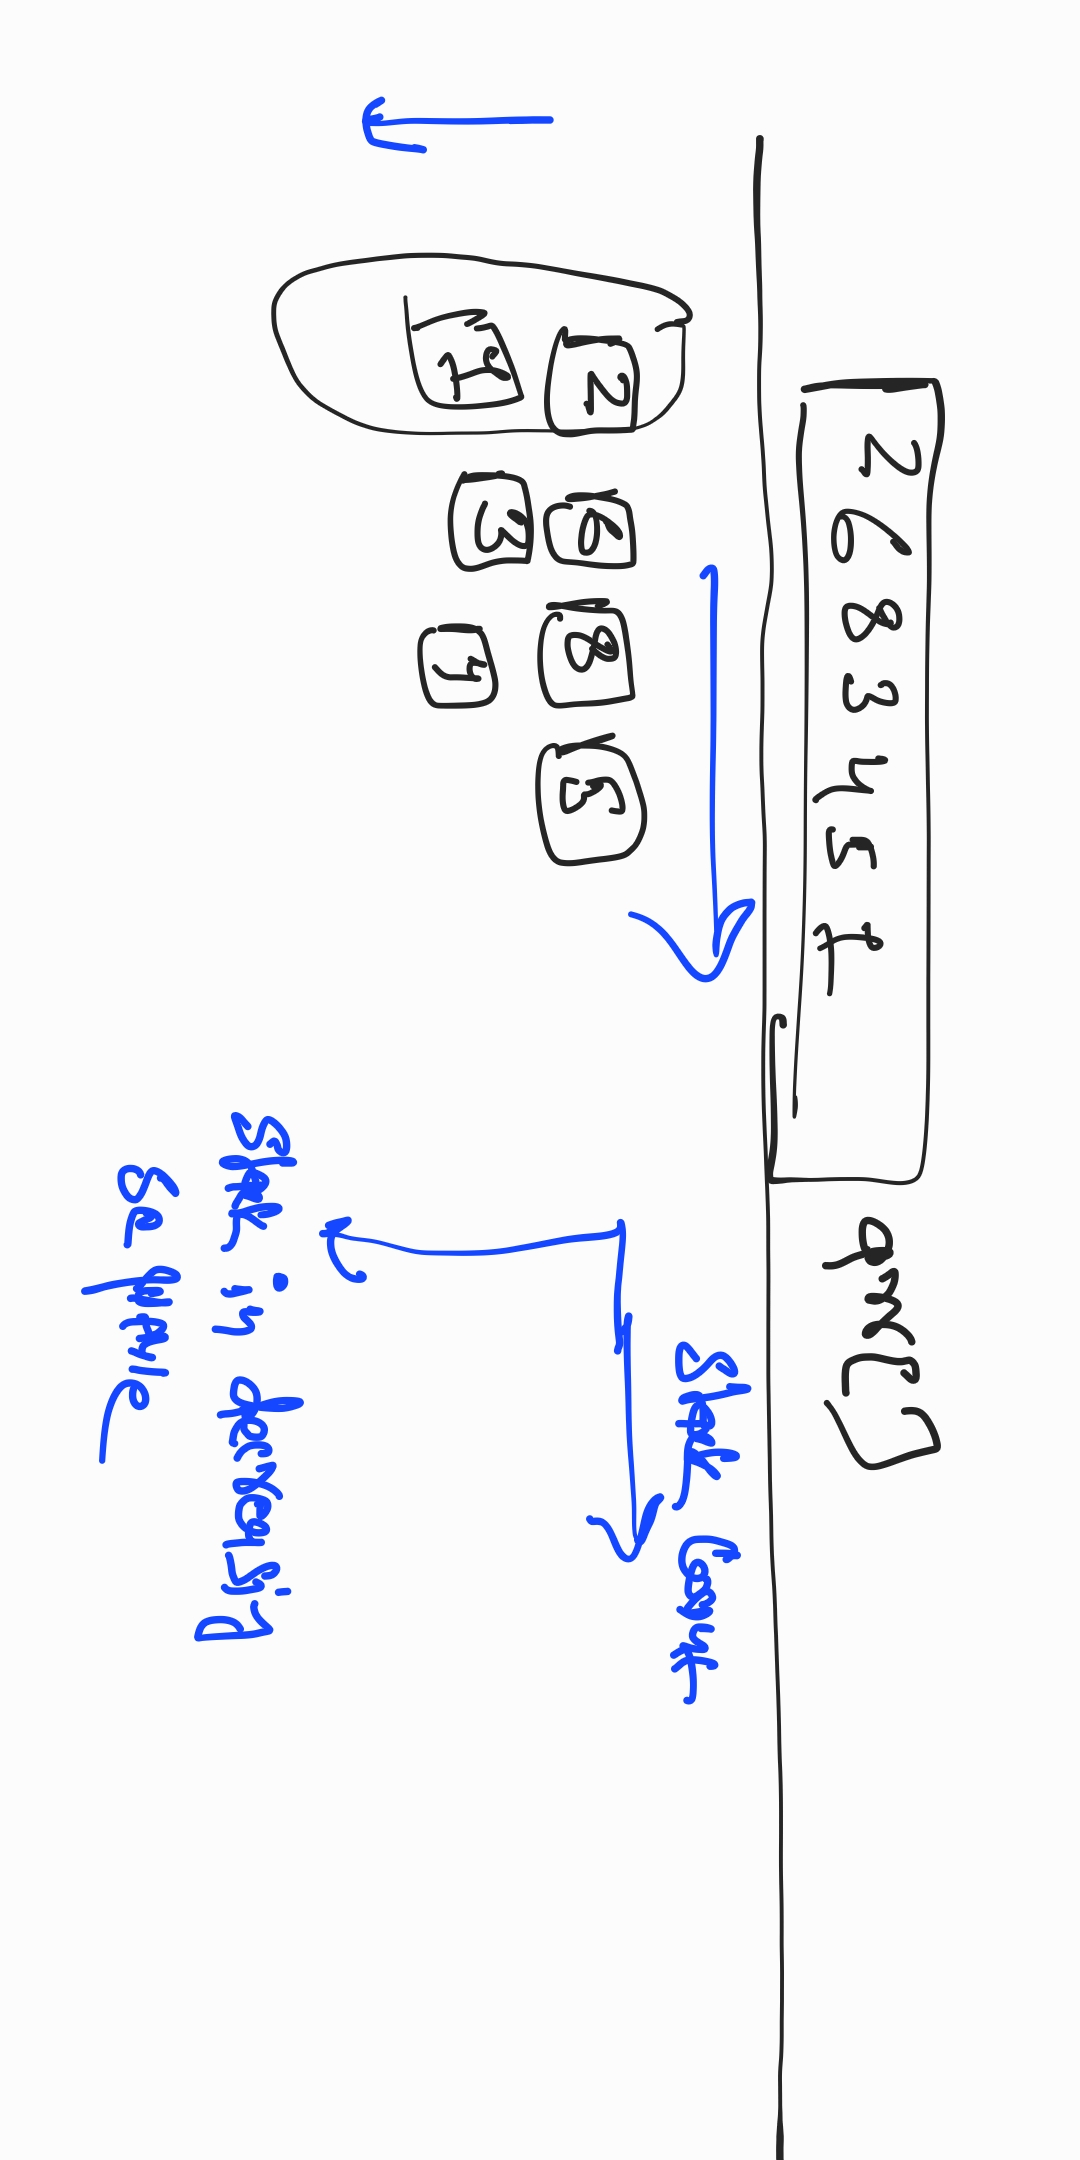
\includegraphics[angle=90,width=9cm,height=5cm]{./resources/PatienceSoring.jpg}
        \caption{Patience Sorting State when all element are processed.}
        \end{figure}
        
        (a) If this card is maximum amoung all the top cards of stack $\implies$ a new stack is created on right side.\\
        (b) If this card can be placed on top of some stack, then we chose the leftmost stack to place it upon.
        
        We keep repeating above operation keeping in mind that our goal is to minimize 

        See file /resource/LISPatienceSoring.pdf for more detail if you require.

    \marginnote{
    \textbf{This is using marginnote!}
        Hello i am from MaringNotes Text. I wonder what else can you place here.
      Is it okay, it its too long???
      
      }

    \begin{verbatim}
    int LICPatienceSorting(vector<int> &arr)
    {
        vector<int> sTop; 
        int size = arr.size();
        
        for(int i=0;i<size;i++)
        {
            int val = arr[i];
            
            //in all available stack, find the stack on which current element can be placed. 
            auto it = lower_bound(sTop.begin(),sTop.end(),val); 

            if(it == sTop.end())
            {
                /*current element is greator than all of the stack's top element => we need to 
                start a new stack*/
                sTop.push_back(val);
            }
            else
            {
                //we found a stack over which we can place the current element => place it on top
                int idx = it - sTop.begin();
            
                sTop[idx] = val; 
            }
        }//for loop ends here
        
        return sTop.size();
    }
    
    \end{verbatim}

\end{solution}

\begin{solution}[using lcs | $O(n^2)$]
    There is one more interesting solution.
    The intution is that if we sort the array (lets call it sortedArr). And then if we find the Longest Common Subsequence
    between arr[] and sortedArray[] then it will be our LongestIncreasingSubsequence!!
\end{solution}

\begin{comment}
    % Below code is not so important, so skipped it
\begin{solution}
    Can you build up a recursive soltion with following defination:
    f(idx,\_):= maximum lis length ending at idx. \textbf{(i.e we must include idx)}

    considering that we know the subproblem answer.
    Then at index idx, we have following option:

    
    val1 = f(1) + 1 IF arr[1] < arr[idx]\\
    val2 = f(2) + 1 IF arr[2] < arr[idx]\\
    \dots\\
    $val_j = f(j) + 1 IF arr[j] < arr[idx] (for all j<idx)$

    we will take the best of all the options.

    Now, for f(idx) can you devise recursive relation?

    Code: see the findAnsFour(), some line in recursive solution is not so intutive.

    
\end{solution}
\end{comment}

% //To-DO Add pratice question environment.
Pratice Questions:
\begin{enumerate}[(i)]
    \item Follow-up question: for patience sorting algorithm. Can you print the LIS in O(n*long(n)) time?
    \item Can you print the patience soring stack, when the the array is [1,2,4,3,5,4,7,2]?
    \item LC2111  Minimum Operations to Make the Array K-Increasing.
    \item LC673  Number of Longest Increasing Subsequence. (First give a $O(n^2)$ solution, then improve it to O(log n)).
\end{enumerate}

\vspace{3cm}
Pratice Question Comment(Possibly hints too):
\begin{enumerate}[(i)]
    \item Follow the image for hint. 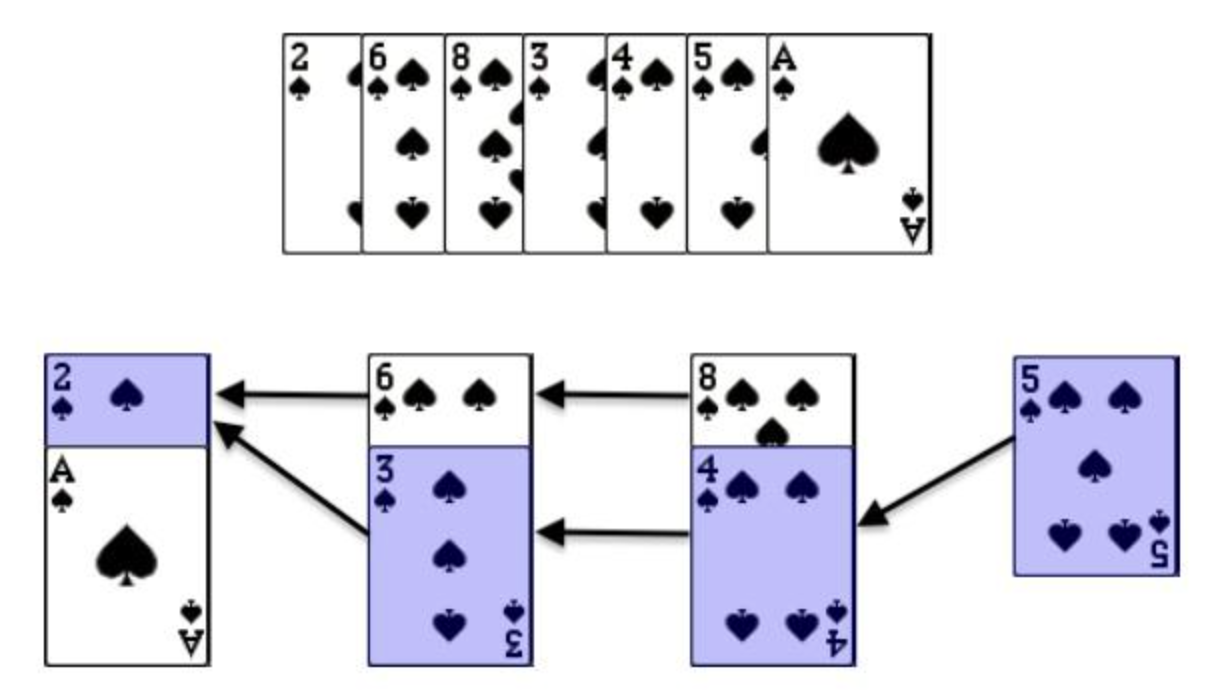
\includegraphics[width=5cm,height=3cm]{./resources/LICSequence.png}
    \item 
    \item LC2111 use $O(log(n))$ to determine LIS length. You can either use PatienceSorting to determine lis lenght in log(n) 
    \item we skipped O(long n) due to its solution complexity.(as at this level you also dont need it)
\end{enumerate}
